\documentclass[main.tex]{subfiles}

\begin{document}

\subsection{Terzo esercizio}

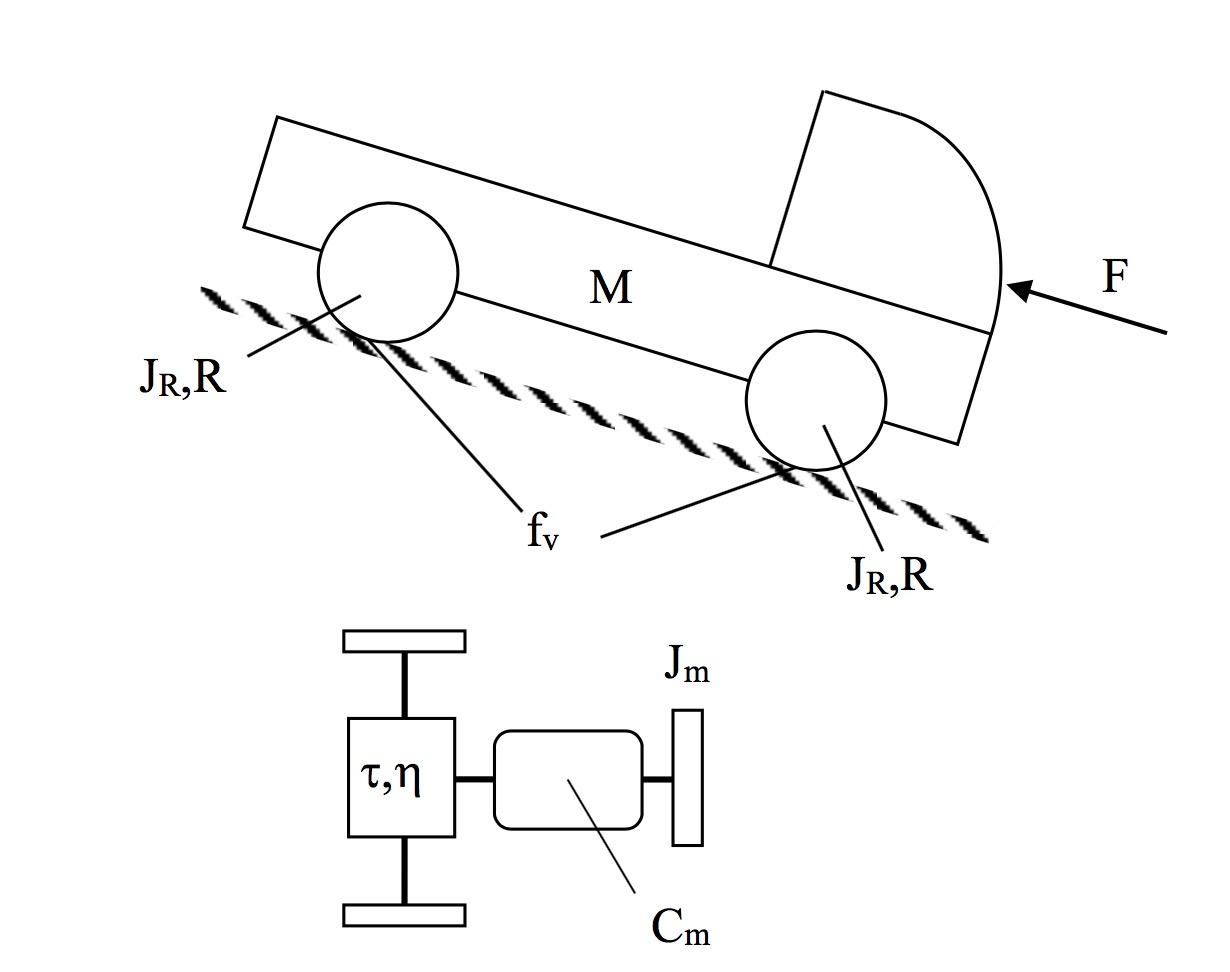
\includegraphics[width=\textwidth]{2015-2207-3.jpg}

\begin{alignat*}{5}
  M=1800\,kg\quad
  \mu_d = 0.9\quad
  J_R = 3\,kgm^2\quad
  \mu_r =0.8\quad
  J_m=0.8\,kg m^2\quad
\end{alignat*}

\begin{alignat*}{5}
  f_v = 0.05\quad
  R = 0.4\,m\quad
  F = 250\,N\quad
 \tau = \frac{1}{4}\quad
 \alpha = 5\deg
\end{alignat*}

Il veicolo rappresentato in figura è posto nel piano verticale ed avanza in discesa lungo un piano inclinato di $\alpha$ rispetto al piano orizzontale. Il veicolo è movimentato tramite un motore longitudinale avente momento d'inerzia $J_m$ e in grado di generare una coppia motrice $C_m$.

Al motore è collegata una trasmissione, di cui sono noti il rapporto di trasmissione $\tau$, il rendimento in moto diretto $\mu_d$ e il rendimento in moto retrogrado $\mu_r$.

Si consideri pari a M la massa totale del veicolo (comprensiva anche della massa delle ruote), pari a R il raggio delle ruote, pari a $J_R$ il momento d'inerzia di ciascuna coppia di ruote (anteriori e posteriori) e pari a $f_v$ il coefficiente di attrito volvente delle ruote stesse.

Sul veicolo agisce una forza aerodinamica $F$, di cui è noto il valore per la velocità di avanzamento assegnata.

Si chiede di calcolare:
\begin{enumerate}
	\item La coppia motrice $C_m$ considerando il veicolo a regime.
	\item La coppia motrice necessaria affinché il veicolo abbia un'accelerazione pari a $0.5\,m/s^2$.
\end{enumerate}

\clearpage

\subsection{Soluzione terzo esercizio}
\subsubsection{Primo punto}

\paragraph{Calcolo della potenza motrice}

\[
	W_m = Cm*\omega_m
\]

\paragraph{Calcolo della potenza resistente} Calcolo per prima cosa la potenza resistente per poter identificare il tipo di moto.

Prendo quindi in considerazioni l'effetto di \textit{forze peso}, \textit{attriti} e \textit{forze applicate}.

\[
	W_{resistente} = M\vec{g}\bullet \vec{v} + \vec{F}\bullet \vec{v} + \vec{F}_v\bullet \vec{v}
\]

La velocità del veicolo è inclinata a $-\alpha$ gradi.
Risolvo il \textbf{prodotto scalare} ed ottengo:

\begin{enumerate}
	\item La forza peso è inclinata verso il basso e forma un angolo di $\dfrac{\pi}{2} - \alpha$ con il vettore velocità.
	\item La forza $F$ e la forza $F_v$ sono orientate in senso opposto rispetto alla velocità, per cui formano un angolo di $\pi$.
\end{enumerate}

\begin{align*}
	W_{resistente} &= Mgv\cos(\dfrac{\pi}{2} - \alpha) + Fv\cos\pi + F_vv\cos\pi \\
	W_{resistente} &= Mgv\sin(\alpha) - Fv - F_vv \\
\end{align*}

Calcolo la forza d'attrito volvente $F_v$:

\begin{align*}
	F_v &=  f_v(N_{ant_{dx}} + N_{ant_{sx}} + N_{pos_{dx}} + N_{pos_{sx}}) \\
\end{align*}

La sommatoria delle forze normali è pari alla componente normale della forza peso del veicolo.

\[
	F_{g_y} = N_{ant_{dx}} + N_{ant_{sx}} + N_{pos_{dx}} + N_{pos_{sx}}
\]

La componente normale della forza peso risulta pari a:

\[
	F_{g_y} = F_g\sin(\dfrac{\pi}{2}+\alpha) = F_g\cos\alpha
\]

\begin{align*}
	F_v &= f_vF_{g_y} = f_vF_g\cos\alpha = f_vMg\cos\alpha
\end{align*}

\begin{align*}
	W_{resistente} &= Mgv\sin(\alpha) - Fv - vf_vMg\cos\alpha \\
\end{align*}

Definisco la velocità $v$ con cui il veicolo si muove sfruttando il legame cinematico con la velocità angolare $\omega_r$ della ruota, che a sua volta è legata con un parametro $\tau$ alla velocità angolare motrice $\omega_m$.

\[v = R\omega_r = R\tau\omega_m\]

Raccolgo la velocità e sostituisco:

\begin{align*}
	W_{resistente} &= R\tau\omega_m(Mg\sin(\alpha) - F - f_vMg\cos\alpha) \\
\end{align*}

Semplifico e raccolgo il coefficiente della forza peso:

\begin{align*}
	W_{resistente} &= R\tau\omega_m(Mg(\sin\alpha - f_v\cos\alpha) - F) \\
\end{align*}



Calcolo il valore del coefficiente:

\[
	Mg(\sin\alpha - f_v\cos\alpha) - F \approx 409 N > 0
\]

Il coefficiente ha segno positivo, e siccome son in condizioni di regime è dimostrazione sufficiente per dire che il moto risulta \textbf{retrogrado}.

\paragraph{Calcolo della potenza perduta}
poiché siamo in condizioni di \textbf{moto retrogrado}, usiamo la formula potenza resistente e $\mu_r$ per calcolare la potenza perduta. Ricordando che siamo in condizioni di regime, la variazione di energia cinetica sarà pari a 0.

\begin{align*}
	W_p &= -(1-\mu_r)(W_r - \dfrac{dEc}{dt}) \\
	W_p &= -(1-\mu_r)W_r \\
\end{align*}

\paragraph{Bilancio delle potenze}
Per calcolare la coppia motrice $C_m$ vado ad usare la formula del \textbf{bilancio delle potenze} ricordando che siamo in condizioni di regime.
\begin{align*}
	W_m + W_r + W_p &= \dfrac{dEc}{dt} \\
	W_m + W_r + W_p &= 0
\end{align*}

\begin{equation}
	C_m\omega_m + W_r  - (1-\mu_r)W_r = 0
\end{equation}

\begin{equation}
	C_m\omega_m + \mu_rW_r = 0
\end{equation}

\begin{equation}
	C_m\omega_m + \mu_rR\tau\omega_m(Mg(\sin\alpha - f_v\cos\alpha) - F) = 0
\end{equation}

\begin{equation}
	C_m + \mu_rR\tau(Mg(\sin\alpha - f_v\cos\alpha) - F) = 0
\end{equation}

\begin{equation}
	C_m = - \mu_rR\tau(Mg(\sin\alpha - f_v\cos\alpha) - F)
\end{equation}

\begin{equation}
	C_m = -32.75\,Nm (C_{m_{riportato}} = 32.8\,Nm)
\end{equation}

\subsubsection{Secondo punto}
Si tratta di calcolare una $C_m$ tale per cui la $a = \dot{\omega}_m\tau R = 0.5\,m/s^2$

\paragraph{Calcolo energia cinetica totale} considero le masse in moto e i momenti di inerzia di masse in rotazione.

\[
	E_c = \dfrac{1}{2}Mv^2 + \dfrac{1}{2}J_m\omega_m^2 + J_R(\tau\omega_m)^2
\]

Sostituisco il legame cinematico della velocità, $v = R\tau\omega_m$:

\[
	E_c = \dfrac{1}{2}M(R\tau\omega_m)^2 + \dfrac{1}{2}J_m\omega_m^2 + J_R(\tau\omega_m)^2
\]

Semplifico l'espressione:

\[
	E_c = \omega_m^2(\dfrac{1}{2}MR^2\tau^2 + \dfrac{1}{2}J_m + J_R\tau^2)
\]

Derivo:

\[
	\dfrac{E_c}{dt} = \omega_m\dot{\omega}(MR^2\tau^2 + J_m + 2J_R\tau^2)
\]

\paragraph{Tipo del moto}
Verifico il tipo del moto tramite la disequazione:

\[
	W_r - \dfrac{dE_{c_r}}{dt} > 0
\]

Se essa vale, allora il moto risulta retrogrado, altrimenti diretto.

\[
	R\tau\omega_m(Mg(\sin\alpha - f_v\cos\alpha) - F) - \omega_m\dot{\omega}_m(MR^2\tau^2 + 2J_R\tau^2) > 0
\]

Semplifico velocità angolare:

\[
	R\tau(Mg(\sin\alpha - f_v\cos\alpha) - F) - \dot{\omega}_m(MR^2\tau^2 + 2J_R\tau^2) > 0
\]

Sfruttando il legame cinematico dell'accelerazione angolare, sostituisco con l'accelerazione fornita, $a = \dot{\omega}_m\tau R \longleftrightarrow \dot{\omega}=\dfrac{a}{\tau R}$:

\[
	R\tau(Mg(\sin\alpha - f_v\cos\alpha) - F) - \dfrac{a}{\tau R}(MR^2\tau^2 + 2J_R\tau^2) > 0
\]

Semplifico nuovamente i termini in comune:

\[
	R(Mg(\sin\alpha - f_v\cos\alpha) - F) - \dfrac{a}{R}(MR^2 + 2J_R) > 0
\]

Sostituisco numericamente ed ottengo:

\[
	-203.7 > 0
\]

La disequazione risulta falsa, quindi il moto è \textbf{diretto}.

\paragraph{Calcolo potenza perduta in moto diretto}

\[
	W_p = -(1-\mu_d)(W_m - \dfrac{dE_{c_m}}{dt}) = -(1-\mu_d)(W_m - Jm\omega_m\dot{\omega}_m)
\]

\paragraph{Applico il bilancio delle potenze}
\[
	W_m + W_r + W_p = \omega_m\dot{\omega}(MR^2\tau^2 + J_m + 2J_R\tau^2)
\]

\[
	W_m + W_r - (1-\mu_d)(W_m - J_m\omega_m\dot{\omega}_m) = \omega_m\dot{\omega}(MR^2\tau^2 + J_m + 2J_R\tau^2)
\]

\[
	W_r +\mu_d(W_m - J_m\omega_m\dot{\omega}_m) = \omega_m\dot{\omega}(MR^2\tau^2 + J_m + 2J_R\tau^2)
\]

\[
	R\tau\omega_m(Mg(\sin\alpha - f_v\cos\alpha) - F) +\mu_d(C_m\omega_m - J_m\omega_m\dot{\omega}_m) = \omega_m\dot{\omega}(MR^2\tau^2 + J_m + 2J_R\tau^2)
\]

Semplifico per $\omega_m$:

\[
	R\tau(Mg(\sin\alpha - f_v\cos\alpha) - F) +\mu_d(C_m - J_m\dot{\omega}_m) = \dot{\omega}(MR^2\tau^2 + J_m + 2J_R\tau^2)
\]

Risolvo per $C_m$:

\[
	R\tau(Mg(\sin\alpha - f_v\cos\alpha) - F) +\mu_dC_m - \mu_dJ_m\dot{\omega}_m = \dot{\omega}(MR^2\tau^2 + J_m + 2J_R\tau^2)
\]

\[
	C_m = \frac{\dot{\omega}(MR^2\tau^2 + J_m + 2J_R\tau^2) + \mu_dJ_m\dot{\omega}_m - R\tau(Mg(\sin\alpha - f_v\cos\alpha) - F)}{\mu_d}
\]

Semplifico quanto possibile l'espressione:

\[
	C_m = \frac{\dot{\omega}(\tau^2 (MR^2+ J_m + 2J_R) + \mu_dJ_m) - R\tau(Mg(\sin\alpha - f_v\cos\alpha) - F)}{\mu_d}
\]

Sostituisco $\dot{\omega}_m =\dfrac{a}{\tau R}$:

\[
	C_m = \frac{\dfrac{a}{\tau R}(\tau^2 (MR^2+ J_m + 2J_R) + \mu_dJ_m) - R\tau(Mg(\sin\alpha - f_v\cos\alpha) - F)}{\mu_d}
\]

Infine sostituisco numericamente:

\[
	C_m = 60.86 Nm \quad (C_{m_{riportato}} = 60.6\,Nm)
\]


\end{document}